\documentclass[12pt, a4paper]{article}

% Ru lang stuff
\usepackage [utf8x] {inputenc}
\usepackage [T2A] {fontenc}

% running titles 
\usepackage{fancybox}
\usepackage{fancyhdr}

% for last page number
\usepackage{lastpage}

%for colored tablets cells
\usepackage{colortbl}

% for Ru text in formulas
\usepackage[warn]{mathtext}

% for captions 
\usepackage[labelsep=period]{caption}
\usepackage{capt-of}

% for colored hyperrefs
\usepackage{xcolor}
\usepackage{hyperref}

% for pictures 
\usepackage{graphicx}

% for coll math
\usepackage{amsmath}

% path to all pictures
\graphicspath{{picks/}}

% for enumerates
\usepackage[shortlabels]{enumitem}

% for diff running titles on pages with diff parity
\usepackage{ifthen}
\usepackage{pdfpages}
\usepackage[strict]{changepage}

%for drawings
\usepackage{tikz}
\usetikzlibrary{calc}
\usetikzlibrary{decorations.pathmorphing}

% for good text in tablets
\usepackage{array}

% upgrading tables
\newcolumntype{P}[1]{>{\centering\arraybackslash}p{#1}}
\newcolumntype{M}[1]{>{\centering\arraybackslash}m{#1}}


% dock fields 20 15 15 35
\usepackage[left=12mm, top=12mm, right=15mm, bottom=28mm, nohead, footskip=10mm]{geometry}

% for cool tables
\usepackage{multirow}

% for different section/subsection/subsubsection styles in contents and doc
\usepackage[english, russian]{babel}

\usepackage{amsmath}

% for cool tables
\usepackage{tabularx}

\newcommand{\sect}[2] {
    \addtocounter{section}{1}
    \section*{\Huge\thesection.\,#1}
    \addcontentsline{toc}{subsection}{ \texorpdfstring{\thesection.\qquad\qquad #2}{Lg}}
}

\newcommand{\subsec}[2] {
    \addtocounter{subsection}{1}
    \subsection*{\thesubsection.\,#1}
    \addcontentsline{toc}{subsection}{ \texorpdfstring{\quad \thesubsection.\qquad\ #2}{Lg}}
}

\newcommand{\subsubsec}[2] {
    \addtocounter{subsubsection}{1}
    \subsubsection*{\thesubsubsection.\,#1}
    \addcontentsline{toc}{subsection}{ \texorpdfstring{\quad\quad\ \thesubsubsection. #2}{Lg}}
}
%-------------------------------------------------------------------------%

% for easy mini pages with shifts
\newcommand{\shiftedText}[3]{
\hspace*{#1}\begin{minipage}[t]{#2}
#3
\end{minipage}
}

\newcolumntype{P}[1]{>{\centering\arraybackslash}p{#1}}

% page style setup (for running titles)
\fancypagestyle{plain}{ %
\fancyhf{} % remove everything

 % lines parameters
\renewcommand{\headrulewidth}{0pt}
\renewcommand{\footrulewidth}{0pt}

% running titles contents
\fancyfoot[L]{\ifthenelse{\isodd{\thepage}}{Работа 1.4.8}{\thepage}}
\fancyfoot[R]{\ifthenelse{\isodd{\thepage}}{\thepage}{Работа 1.4.8}}
}

% choosing page style with our running titles
\pagestyle{plain}

\tolerance = 10000

\title{Лабораторная работа №1.4.8}
\author{Mikhail Pavlov \thanks{MIPT}}
\date{November, 2021}
\begin{document}


\shiftedText{0.5cm}{14cm}
{
    \begin{center}
    \vspace*{1.0cm}    
        
        {\bf\Huge Работа 1.4.8 }
        
    \vspace*{0.2cm}    
        
        {\bf\LARGE Измерение модуля Юнга методом акустического резонанса. }
        
    \vspace*{0.8cm}
        {\LARGE Работу выполнил Павлов Михаил Б01-109 }
        
    \vspace*{1.6cm}
    
    \end{center}
}

\fancypagestyle{plain}{ %
\fancyhf{} % remove everything

 % lines parameters
\renewcommand{\headrulewidth}{0pt}
\renewcommand{\footrulewidth}{0pt}
% running titles contents
\fancyfoot[L]{\ifthenelse{\isodd{\thepage}}{Работа 1.4.8}{\thepage}}
\fancyfoot[R]{\ifthenelse{\isodd{\thepage}}{\thepage}{Работа 1.4.8}}
}

% choosing page style with our running titles
\pagestyle{plain}

\tolerance = 10000

\vspace*{0.6cm}

{\Large 1. Аннотация \\}

Основная цель данной лабораторной работы - поиск модуля Юнга для стержней различных материалов.
Это осуществляется с помощью осциллографа, а именно экспериментатор находит такую частоту
акустических колебания стержня, при которой возникает акустический резонанс, т.е. резкое увеличение амплитуды.
С помощью найденной  частоты и измеренной длины стержней находится скорость акустических волн.
Далее с помощью небольших цилиндров того же материала с высокой точностью измеряется плотность.
Зная плотность материала и скорость волны, можно уже получить модуль Юнга для наших стержней.

\vspace{1cm}
{\Large 2. Теоретические сведения \\}

{\large Введение \\}

Основной характеристикой упругих свойств твёрдого тела является его
модуль Юнга $E$. Согласно закону Гука, если к элементу среды приложено
некоторое механическое напряжение $\sigma$, действующее вдоль некоторой
оси $x$ (напряжения по другим осям при этом отсутствуют), то в этом элементе возникнет относительная деформацию вдоль этой же оси
$\varepsilon = \Delta x/x_0$, определяемая соотношением

\begin{equation}
    \sigma = \varepsilon E
\end{equation}

Если с помощью кратковременного воздействия в некотором элементе
твёрдого тела создать малую деформацию, она будет далее распространяться в среде в форме волны, которую называют акустической или звуковой. Распространение акустических волн обеспечивается за счёт упругости
и инерции среды. Волны сжатия/растяжения, распространяющиеся вдоль
оси, по которой происходит деформация, называются продольными. Как
будет строго показано далее, скорость $u$ распространения продольной акустической волны в простейшем случае длинного тонкого стержня определяется соотношением

\begin{equation}
    u = \frac{E}{\rho},
\end{equation}
где $\rho$ --- плотность среды.
			
Рассмотрим стержень постоянного круглого сечения, радиус $R$ которого
много меньше его длины $L$. С точки зрения распространения волн стержень
можно считать тонким, если длина $\lambda$ звуковых волн в нём велика по сравнению с его радиусом: 
$\lambda >> R$. Такая волна может свободно распространяться только вдоль стержня, поэтому можно считать, 
что стержень испытывает деформации растяжения и сжатия только вдоль своей оси.

Акустическая волна, распространяющаяся в стержне конечной длины $L$,
испытает отражение от торцов стержня. Если при этом на длине стержня
укладывается целое число полуволн, то отражённые волны будут складываться в фазе с падающими, что приведёт к резкому усилению амплитуды
их колебаний и возникновению акустического резонанса в стержне. Измеряя соответствующие резонансные частоты, можно определить скорость
звуковой волны в стержне и, таким образом, измерить модуль Юнга материала стержня. Акустический метод является одним из наиболее точных
методов определения упругих характеристик твёрдых тел.

{\large Уравнение волны в тонком стержне \\}

Получим дифференциальное уравнение, описывающее распространение упругих волн в тонком стержне.
Направим ось $x$ вдоль геометрической оси стержня (рис. 1). Разобьём
исходно недеформированный стержень на тонкие слои толщиной $\Delta x$. При
продольной деформации среды границы слоёв сместятся в некоторые новые положения. Пусть плоскость среды, находящаяся исходно в точке $x$,
сместилась к моменту $t$ на расстояние $\xi(x,t)$. 
Тогда слой, занимавший исходно отрезок $[x; x + \Delta x]$, изменил свой продольный размер на величину
$\Delta \xi = \xi(x + \Delta X,t) − \xi(x,t)$. Пользуясь малостью $\Delta x$ и определением производной, получим $\Delta \xi = \frac{\partial\xi}{\partial x} \Delta x$. 
Таким образом, функция

\begin{equation}
    \varepsilon = \frac{\partial\xi}{\partial x}
\end{equation}
это относительное удлинение элемента стержня в точке $x$.

Заметим, что смещение слоёв $\xi(x,t)$ является функцией не только координаты, но и времени, 
поэтому мы используем обозначения для частных производных по координате и времени.

Далее, согласно закону Гука, имеем

\noindent\begin{minipage}[c]{0.4\textwidth}
    \hspace{1cm}
    \begin{equation}
        \sigma = \varepsilon E = E\frac{\partial\xi}{\partial x}
    \end{equation}
    Здесь напряжение равно $\sigma = F\S$, где $F$ --- продольная сила, действующая на элементарный
    участок $\Delta x$, $S$ --- площадь поперечного сечения стержня.

    Напряжения, действующие
    на стенки рассматриваемого
    элемента в сечениях $x$ и $x + \Delta x$,
    будут различными. Из-за этого
    возникнет результирующая возвращающая сила, стремящаяся
    вернуть элемент стержня в исходное (недеформированное и
    несмещённое) состояние:

\end{minipage}
\begin{minipage}[c]{0.57\textwidth}
    \begin{center}
        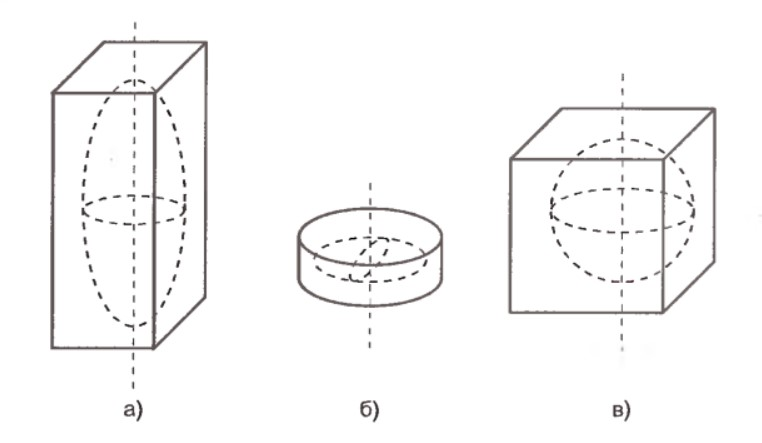
\includegraphics[scale=0.58]{Pics/picture1.jpg} \\
        \textit{\textcolor[HTML]{000000}{Рис. 1. Силы, действующие на элемент стержня при продольных колебаниях}}
    \end{center}
\end{minipage}  

\begin{equation}
    \Delta F = S\sigma(x + \Delta x) - S\sigma(x) = \frac{\partial\sigma}{\partial x} S\Delta x = \frac{\partial^2\xi}{\partial x^2}ES\Delta x.
\end{equation}

Эта сила вызовет ускорение движение элемента стержня массой $\Delta m = S\rho\Delta x$ вдоль оси $x$. Ускорение рассматриваемого элемента --- это вторая
производная по времени от смещения его границ: 

\begin{displaymath}
    a = \frac{\partial^2\xi}{\partial t^2}
\end{displaymath}
Тогда используя 2-ой закон Ньютона и соотношения (3) - (5), получим уравнение движения среды:

\begin{displaymath}
    S\rho\Delta x\frac{\partial^2\xi}{\partial t^2} = SE\Delta x\frac{\partial^2\xi}{\partial x^2}.
\end{displaymath}

Наконец, вводя величину с размерностью скорости согласно (2), запишем полученное уравнение в окончательном виде:

\begin{equation}
    \frac{\partial^2\xi}{\partial t^2} = u^2\frac{\partial^2\xi}{\partial x^2}
\end{equation}

Это уравнение носит название волнового. Оно имеет универсальный характер и описывает волны самой разной природы: акустические волны в
твёрдых телах, жидкостях и газа, волны на струне, электромагнитные
волны и т.п. Как будет показано далее, величина $u$ в уравнении (6) имеет
смысл скорости распространения волны.

\vspace{1cm}
{\large Бегущие акустические волны. Скорость волны \\}

Покажем, что произвольная функция вида $\xi(x,t) = \phi(x - ut)$ --- то есть
функция, зависящая только от комбинации $X = x - ut$, — является решением волнового уравнения (6). Действительно, прямой подстановкой в (6),
используя формулу производной сложной функции, убеждаемся, что волновое уравнение обращается в тождество при любой функции $\phi$:

\begin{displaymath}
    \frac{\partial^2\phi}{\partial t^2} \equiv u^2 \frac{\partial^2\phi}{\partial x^2}
\end{displaymath}

Как показывается в математических курсах,
общее решение дифференциального уравнения (6) представимо в 
виде суммы двух волн произвольной формы, бегущих в противоположные
стороны со скоростями $\pm u$:

\begin{equation}
    \xi(x,t) = \phi_1(x - ut) + \phi_2(x + ut),
\end{equation}
где $u$ --- скорость волны, $\phi_1$ и $\phi_2$ --- функции, вид которых в конкретной задаче
определяется из начальных и граничных условий.

\vspace{1cm}
{\large Собственные колебания стержня. Стоячие волны \\}

В случае гармонического возбуждения колебаний с частотой $f$ продольная волна в тонком стержне может быть представлена 
в виде суперпозиции двух бегущих навстречу гармонических волн:

\begin{equation}
    \xi(x,t) = A_1sin(\omega t - kx + \varphi_1) + A_2sin(\omega t + kx + \varphi_2),
\end{equation}
где $\omega = 2 \pi f$ --- циклическая частота. Коэффициент $k$ называют
волновым числом или пространственной частотой волны. 

Далее, перепишем исследуемую функцию (8), используя граничные
условия равенства амплитуд и фазы и формулу суммы синусов:

\begin{equation}
    \xi(x,t) = 2Acos(kx)sin(\omega t + \varphi).
\end{equation}
Колебания вида (9) называют гармоническими стоячими волнами.

Наконец, воспользовавшись вторым граничным условием, придем к уравнению
$sin kL = 0$, решения которого определяют набор допустимых значений волновых чисел $k$.
Выражая это все через длину волны $\lambda$, получим 

\begin{equation}
    \lambda_n = \frac{2L}{n}, n \in N
\end{equation}
Таким образом, для возбуждения стоячей волны на длине стержня должно
укладываться целое число полуволн.

Допустимые значения частот

\begin{equation}
    f_n = \frac{u}{\lambda_n} = n\frac{u}{2L}, n \in N
\end{equation}
называют собственными частотами колебаний стержня длиной $L$.
Именно при совпадении внешней частоты с одной из частот $f_n$ в стержне
возникает акустический резонанс.

Точки с максимальной амплитудой называются пучностями смещения, точки с минимальной
(нулевой) амплитудой --- узлами смещения. Номер гармоники $n$ определяет количество узлов смещения на стержне. 
Заметим, что согласно закону Гука (1) в пучности смещения имеет место узел напряжения, и, наоборот,
в узлах смещения имеется пучность напряжения (в частности, на свободных торцах стержня напряжение всегда нулевое, а деформация максимальна).

\vspace{1cm}
{\Large 3. Экспериментальная установка \\}

\begin{center}
    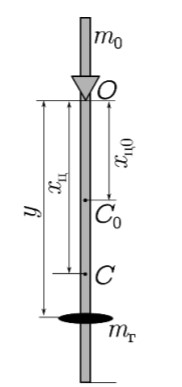
\includegraphics[scale=0.9]{Pics/picture2.jpg} \\
    \textit{\textcolor[HTML]{000000}{Рис. 2. Схема установки: 1 --- генератор звуковой частоты, 2 --- частотомер,
    3 --- осциллограф, 4 --- электромагнит-возбудитель, 5 --- образец, 6 --- электромагнитприёмник, 7 --- усилитель звуковой частоты, 8 --- блок питания усилителя,
    9, 11 --- стойки крепления электромагнитов, 10 --- стойка крепления образца, 12 --- направляющая}}
\end{center}

Схема экспериментальной установки приведена на рис. 2. Исследуемый
стержень 5 размещается на стойке 10. Возбуждение и приём колебаний в
стержне осуществляются электромагнитными преобразователями 4 и 6,
расположенными рядом с торцами стержня. Крепления 9, 11 электромагнитов дают возможность регулировать их расположение по высоте, а
также перемещать вправо-влево по столу 12.

Электромагнит 4 служит для возбуждения упругих механических продольных колебаний в стержне. На него с генератора звуковой частоты 1 подаётся сигнал синусоидальной формы: 
протекающий в катушке электромагнита ток создаёт пропорциональное ему магнитное поле, вызывающее
периодическое воздействие заданной частоты на торец стержня (к торцам
стержней из немагнитных материалов прикреплены тонкие стальные
шайбы). Рядом с другим торцом стержня находится аналогичный электромагнитный датчик 6, который служит для преобразования механических
колебаний в электрические. Принцип работы электромагнитных датчиков
описан подробнее ниже.

Сигнал с выхода генератора поступает на частотомер 2 и на вход
канала X осциллографа 3. ЭДС, возбуждаемая в регистрирующем электромагните 6, пропорциональная амплитуде колебаний торца стержня, усиливается усилителем 7 и подаётся на вход канала Y осциллографа.

Изменяя частоту генератора и наблюдая за амплитудой сигнала с регистрирующего датчика, можно определить частоту акустического резонанса
в стержне. Наблюдения в режиме X–Y позволяют сравнить сигналы генератора и датчика, а также облегчает поиск резонанса при слабом сигнале.

{\Large 4. Инструментальные погрешности \\}
\textbf{Линейка: } $\sigma_{rul} = \pm 0.5$ мм (половина цены деления)\\
\textbf{Электронные весы: } $\sigma_{v} = \pm 10^{-3}$ г (маркировка производителя) \\
\textbf{Штангенциркуль: } $\sigma_{cal} = \pm 0.1$ мм (маркировка производителя) \\
\textbf{Частотомер: } $\sigma_{f} = \pm 0.5$ Гц (маркировка производителя) \\


\vspace*{0.3cm}
{\Large 5. Результаты измерений и обработка данных \\} 

Измерим линейные размеры и массу образцов из меди, стали и дюраля. Данные занесем в таблицу 2. 
Вычислим плотность материалов, воспользовавшись формулой $\rho = \frac{m}{V} = \frac{4m}{\pi d^2h}$

\begin{table}[h!]
\centering

\begin{tabular}{|c|c|c|c|c|c|}
\hline
 & \textit{m}, г& h, см& d, см& $\rho$, г/см$^3$& $\delta\rho$, г/см$^3$\\
\hline
Медь & 39.417& 3.97& 1.20& $8.78$& $ 0.03$\\
\hline
Сталь & 37.106& 4.13& 1.20& $7.95$& $ 0.03$\\
\hline
Дюраль & 11.794& 4.03& 1.16& $2.76$& $ 0.03$\\
\hline
\end{tabular}
\label{table2}
\caption{Параметры образцов}
\end{table}

Зависимость частоты от номера резонансного пика для трех измеряемых стержней занесем в Таблицу 2:
\begin{table}[h!]
\begin{center}
\caption{Резонансные частоты стержней}
\begin{tabular}{|c|c|c|c|c|c|c|c|c|}
\hline
 &n &1 &2 &3 &4 &5 &6 &1/2 \\
\hline
 Медь& \textit{f}, кГц& 3.160& 6.297& 9.486& 12.658& 15.806& 18.972& - \\
\hline
 Сталь& \textit{f}, кГц& 4.132& 8.268& 12.394& 16.524& 20.647& 24.771& 2.066 \\
\hline
 Дюраль& \textit{f}, кГц& 4.235& 8.473& 12.702& 16.935& 21.164& 25.383& 2.118 \\
\hline
\end{tabular}
\end{center}
\end{table}

По полученной таблице можем построить график зависимости собственной частоты стержня
от номера гармонии.

\begin{center}
    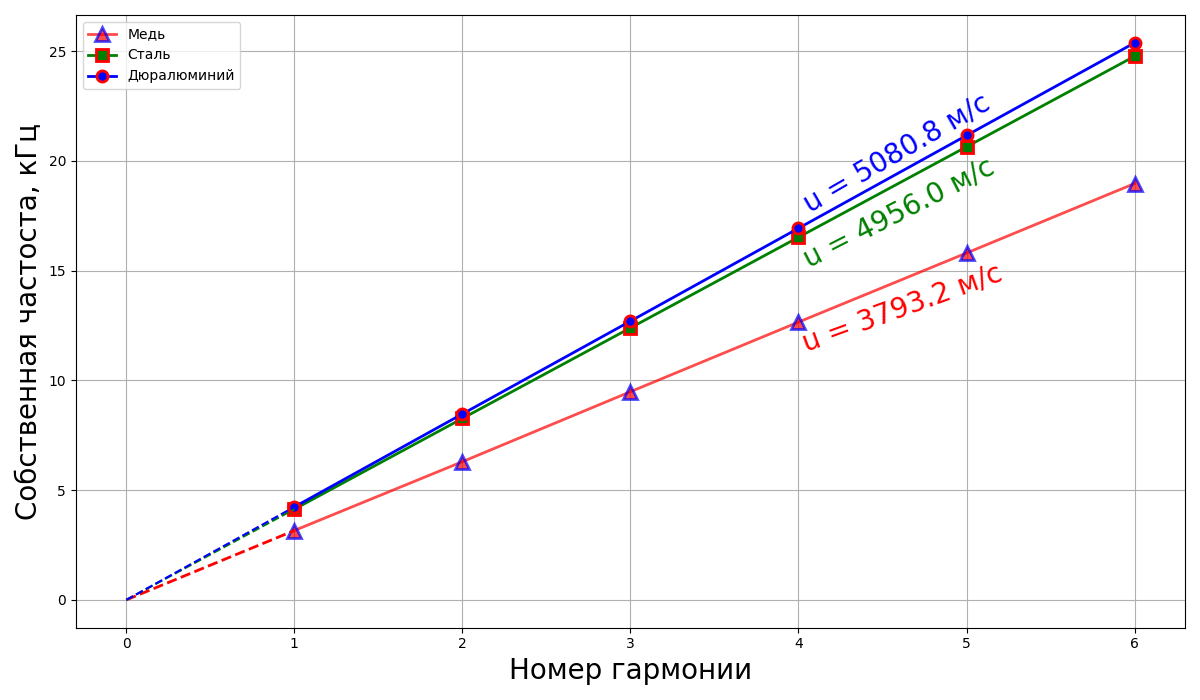
\includegraphics[scale=0.4]{Pics/Picture3.png} \\
    \textit{\textcolor[HTML]{000000}{Рис. 3. График зависимости частоты от номера гармонии}}
\end{center}

Далее методом наименьших квадратов получаем:
\begin{table}[h!]
\begin{center}
\caption{Скорости звука в стержнях}
\begin{tabular}{|c|c|c|c|c|}
\hline
 & $\textit{f}_1$, кГц& $\delta\textit{f}_1$, кГц& $u_{CT}$, м/c& $\delta u_{CT}$, м/c\\ 
\hline
 Медь& 3.161& $2 \cdot 10^{-3}$& 3793.2& 33\\
\hline 
 Сталь& 4.130& $2 \cdot 10^{-3}$& 4956.0& 35\\
\hline 
 Дюраль& 4.234& $2 \cdot 10^{-3}$& 5080.8& 36\\
\hline 
\end{tabular}
\end{center}
\end{table}

Вычислим и занесем в Таблицу 4 модули Юнга материалов:

\begin{table}[h!]
\begin{center}
\begin{tabular}{|c|c|c|c|c|}
    \hline
    & E, ГПа& $\delta$E, ГПа& $E_{tbl}$, ГПа& $|E_{tbl}-E|$, ГПа\\
    \hline
     Медь& 126.3 & 3& 105-130& 0\\
    \hline
     Сталь& 195.3& 5&  200-210& 4.7\\
    \hline
     Дюраль& 71.3& 2& 70.5& 0.8\\
    \hline
    \end{tabular}
    \caption{Модули Юнга}
\end{center}
    \end{table}

    \vspace*{0.3cm}
    {\Large 6. Вывод \\} 

    Таким образом, все значения модуля Юнга в пределах погрешности совпали
    с табличными, поэтому метод акустического резонанса для металлов 
    в целом можно назвать точным и надежным.

\end{document}